

\documentclass{beamer}


% Setup appearance:

\usetheme{Darmstadt}
\usefonttheme[onlylarge]{structurebold}
\setbeamerfont*{frametitle}{size=\normalsize,series=\bfseries}
\setbeamertemplate{navigation symbols}{}


% Standard packages

\usepackage[english]{babel}
\usepackage[latin1]{inputenc}
\usepackage{times}
\usepackage[T1]{fontenc}


% Setup TikZ

\usepackage{tikz}
\usetikzlibrary{arrows}
\usetikzlibrary{calc}
\usepackage{pgfmath}
\usepackage{verbatim}
\usepackage{listings}
\tikzstyle{block}=[draw opacity=0.7,line width=1.4cm]


% Author, Title, etc.

\title[Monitor Platform Architecture Specs] 
{%
Monitor Platform Architecture Spec %
}

\author[Sinha N]
{
  Nish~Sinha\inst{1} \and
}

\institute[Xad]
{
  \inst{1}%
  Xad Inc., Mountain View, USA
  \and
  \vskip-2mm
}

\date[\today]
{\today}



% The main document

\newcommand{\drawLinkArrow}[4]{
		\pgfmathparse{2pt+3.5pt}
	%\draw[->] let
		%\p1 = ($(#1)), \p2 = ($(#2)),
		%\p3 = ($(#3)), \p4 = ($(#4)) 
		%in ($ (\x1 + \x2)*1/2$ ,\y1) -| ($ (\x3 + \x4)*1/2$ ,\y4);
	\draw[->] let
		\p1 = (#1), \p2 = (#2),
		\p3 = (#3), \p4 = (#4)
		in
		({(\x1 + \x2)*1/2} ,\y1) -- ({(\x3 + \x4)*1/2} ,\y4);
}

\newcommand{\drawBox}[3]{
		\shade[top color=yellow,bottom color=black] (#1) rectangle (#2) node[midway,below] {#3};
}

\begin{document}

\begin{frame}
  \titlepage
\end{frame}

\begin{frame}{Outline}
  \tableofcontents
\end{frame}


\section{Introduction}

\subsection{The Architecture}

\begin{frame}{Schema}
   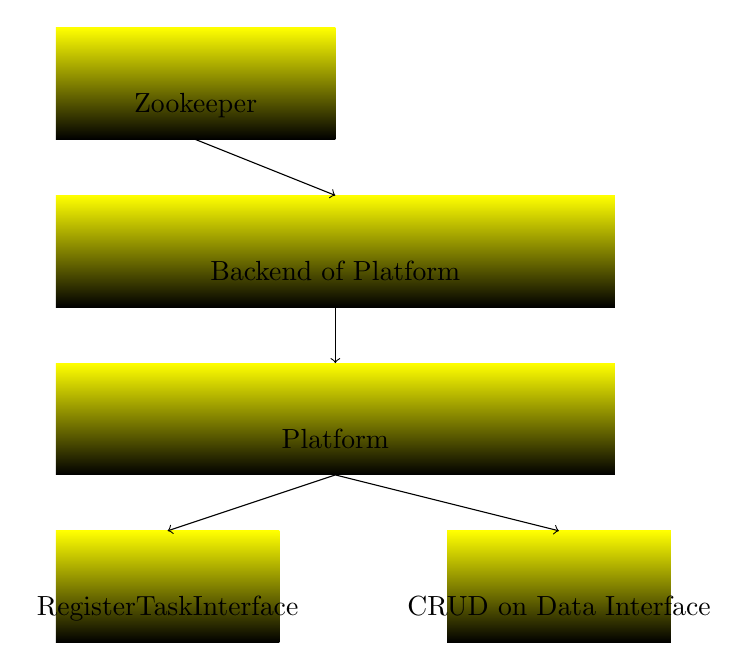
\begin{tikzpicture}[scale=0.71]
     
	\coordinate (B1_L) at (0,0);
	\coordinate (B1_R) at (5,2);
	\coordinate (B2_L) at (0,-3);
	\coordinate (B2_R) at (10,-1);
	\coordinate (B3_L) at (0,-6);
	\coordinate (B3_R) at (10,-4);
	\coordinate (B4_L) at (0,-9);
	\coordinate (B4_R) at (4,-7);
	\coordinate (B5_L) at (7,-9);
	\coordinate (B5_R) at (11,-7);
	\drawBox{B1_L}{B1_R}{Zookeeper}
	\drawBox{B2_L}{B2_R}{Backend of Platform}
	\drawBox{B3_L}{B3_R}{Platform}
	\drawBox{B4_L}{B4_R}{RegisterTaskInterface}
	\drawBox{B5_L}{B5_R}{CRUD on Data Interface}
	\drawLinkArrow{B1_L}{B1_R}{B2_L}{B2_R}
	\drawLinkArrow{B2_L}{B2_R}{B3_L}{B3_R}
	\drawLinkArrow{B3_L}{B3_R}{B4_L}{B4_R}
	\drawLinkArrow{B3_L}{B3_R}{B5_L}{B5_R}

  \end{tikzpicture}

\end{frame}

\section{Interfaces of Platform}
\subsection {RegisterTaskInterface}
\begin{frame}
	\begin{block}{RegisterTaskInterface}
		\begin{itemize}
			\item bool \alert{RegisterTask}(Namespace, PlatformTask(initFn,quitFn,runnableMainTask,CallFrequencyConfig)).
			\begin{itemize}
				\item Namespace(name: String, access:Enum\{exclusive, inclusive\}).
				\item CallFrequnecyConfig(Type: Enum\{periodic,watchOnEvent\}), period: milliseconds).
			\end{itemize}
		\end{itemize}
	\end{block}
\end{frame}


\subsection {DataInterface}
\begin{frame}
\begin{block}{DataInterface}
		\begin{itemize}
			\item bool \alert{createData}(key:String,value:String)
			\item bool \alert{updateData}(key:String,value:String)
			\item bool \alert{deleteData}(key:String)
			\item bool \alert{existsData}(key:String)
			\item String \alert{readData}(key:String)
			\item bool \alert{watchData}(key:Stringi, fn: Function)
		\end{itemize}
	\end{block}

\end{frame}


\subsection {Backend Interface of Platform}
\begin{frame}
   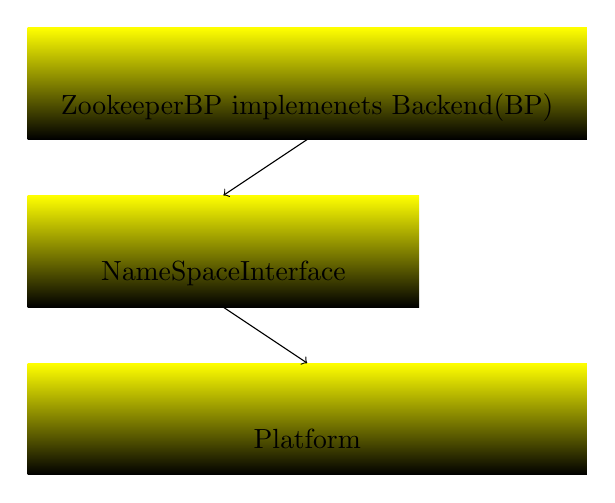
\begin{tikzpicture}[scale=0.71]
     
	\coordinate (B1_L) at (0,0);
	\coordinate (B1_R) at (10,2);
	\coordinate (B2_L) at (0,-3);
	\coordinate (B2_R) at (7,-1);
	\coordinate (B3_L) at (0,-6);
	\coordinate (B3_R) at (10,-4);

	\drawBox{B1_L}{B1_R}{ZookeeperBP implemenets Backend(BP)}
	\drawBox{B2_L}{B2_R}{NameSpaceInterface}
	\drawBox{B3_L}{B3_R}{Platform}
	\drawLinkArrow{B1_L}{B1_R}{B2_L}{B2_R}
	\drawLinkArrow{B2_L}{B2_R}{B3_L}{B3_R}

  \end{tikzpicture}
\end{frame}


\subsection {BackendInterface}
\begin{frame}
\begin{block}{BackendInterface}
		\begin{itemize}
			\item bool \alert{createNamespace}(name:String)
			\item bool \alert{deleteNamespace}(name:String)
			\item bool \alert{setNamespace}(name:String)
			\item bool \alert{exclusiveAccessNamespace}(fn:callbackFn)
			\item bool \alert{inclusiveAccessNamespace}(fn:callbackFn)
			\item bool \alert{createDataNamespace}(key:String)
			\item bool \alert{deleteDataNamespace}(key:String)
			\item bool \alert{watchDataNamespace}(key:String)
			\item String \alert{readDataNamespace}(key:String)
			\item bool \alert{checkDataNamespace}(key:String)
			\item bool \alert{updateDataNamespace}(key:String)
		\end{itemize}
	\end{block}

\end{frame}





\subsection {Example}

\begin{frame}{AWS capacity application}
  \begin{example}
	\begin{itemize}
		\item Consists of two tasks: A leader task and a follower task.
			\begin{itemize}
				\item LeadTask is exclusive on the namespace, and node running it is responsible for quering ELB and populating the namespace with relevant data.
				\item FollowTask is inclusive on the namespace, and every node running it is responsible for quering namespace and for maintaining the local cache in coherence. 
				\item \alert{There is no application level coupling between these two tasks. We will see in a later example why that might be important.}.
			\end{itemize}
	\end{itemize}
	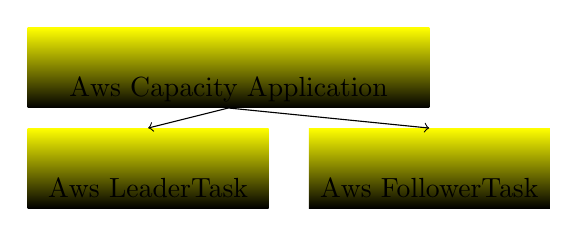
\begin{tikzpicture}[scale=0.51]
		\coordinate (B1_L) at (0,0);
		\coordinate (B1_R) at (10,2);
		\coordinate (B2_L) at (0,-2.5);
		\coordinate (B2_R) at (6,-0.5);
		\coordinate (B3_L) at (7,-2.5);
		\coordinate (B3_R) at (13,-0.5);

		\drawBox{B1_L}{B1_R}{Aws Capacity Application}
		\drawBox{B2_L}{B2_R}{Aws LeaderTask}
		\drawBox{B3_L}{B3_R}{Aws FollowerTask}
		\drawLinkArrow{B1_L}{B1_R}{B2_L}{B2_R}
		\drawLinkArrow{B1_L}{B1_R}{B3_L}{B3_R}

  	\end{tikzpicture}

  \end{example}
\end{frame}

\begin{frame}{AWS capacity application}
	\tiny
	\begin{itemize}
		\item LeaderTask:\texttt{RegisterTask(Namespace(ZK::AWSCAPACITY,
exclusive),new PlatformTask(initFn = () => (),
			quitFn = ()=>(), CallFrequencyConfig(periodic,60000)), def task = ()=> {
	pollAws();
	enumerateActiveNodes();
	foreach node in ActiveNodes :createdata(node,metastate)	
})
 }
	\item FollowerTask:\texttt{RegisterTask(Namespace(ZK::AWSCAPACITY,
inclusive),new PlatformTask(initFn = () => (),
			quitFn = ()=>(), CallFrequencyConfig(watch,-1)), def task = () => {
	x: String= readData(""); //x will contain a list of name of nodes  inside the nmaespace watched
	updateLocalDataStructures();
})
 }

	\end{itemize}
\end{frame}








\appendix

\section*{Appendix}


\end{document}

